\chapter{Koordinatensysteme im Lochkamermodell}
\label{sec:basisTransformation} 

(Neue Einleitung schreiben)
 
In diesem Kapitel wird der Fokus auf die benötigten Koordinatensysteme für die Stereobildanalyse gelegt. Als aller erstes werden anhand praxisnaher Beispiele die Notwendigkeit der Basis Transformation und damit einhergehend der Spezialfall einer Transformation von einem Koordinatensystem wie zum Beispiel einem dreidimensionalen Weltkoordinatensystem $(O,\delta)$ mit $\delta=(\hat{d_1}, \hat{d_2},\hat{d_3},O)$ in ein dreidimensionales Kamerakoordinatensystem $(C,\beta)$ mit $\beta=(\hat{b_1},\hat{b_2},\hat{b_3},C)$ aufgezeigt. Die gewählte Notation zur Beschreibung der Koordinatensysteme setzt sich am Beispiel des Kamerakoordinatensystem aus der Bezeichnung für den Ursprung $C$ und den entsprechenden Koordinatenachsen $(\hat{b_1},\hat{b_2},\hat{b_3})$ mit wiederum $\hat{b_1} = \begin{pmatrix}b_{11}\\b_{12}\\b_{13}\end{pmatrix}$, $\hat{b_2} = \begin{pmatrix}b_{21}\\b_{22}\\b_{23}\end{pmatrix}$ und $\hat{b_1} = \begin{pmatrix}b_{31}\\b_{32}\\b_{33}\end{pmatrix}$, welche mit $\beta$ zusammengefasst werden. In Abbildung \ref{fig:Koordinatensysteme1} sind die beiden kartesischen Koordinatensysteme $(O,\delta)$ und $(C,\beta)$ schematisch dargestellt. 

% werden zunächst ein paar Grundlegende mathematische Operationen vorgestellt, welche das Grundgerüst der Stereokalibrierung und Szenenrekonstruktion bilden.
%
%Noch anzumerken ist, dass in dieser Arbeit grundlegend von orthogonalen Koordinatensystemen ausgegangen wird, andernfalls wird explizit darauf hingewiesen. 
%
%

%\section{Die Transformation von Koordinaten schließt die Transformation der Basis mit ein}
%
%Es sei \textit{V} ein \textit{n}-Dimensionaler Vektorraum über einem Körper \textit{K}. \textit{K} stellt in diesem Beispiel das Skalar \ensuremath{\mathbb{R}} dar, welches alle reelen Zahlen mit einschließt. Zur Veranschaulichung wird der Vektorraum  \ensuremath{V^3} also ein 3-Dimesnionaler Raum gewählt, dessen Basis mit \ensuremath{\beta = [\vec{b}_1, \vec{b}_3, \vec{b}_3]} bezeichnet wird.\cite{Elements} ....  (FORTFÜHREN)\\
%
%A vector $\vec{v} \in V^3$ is uniquely expressed as a linear combination of basic vectors of V 3 by its coordinates $(x,y,z) \in \mathbb{R}$. $\vec{v} = xb_1+yb_2+zb_3$ and can be represented as an ordered triple of coordinates, $\vec{v}_\beta =[x\,y\,z]^T$

\section{Koordinatentransformation durch Basistransformationen}

Anhand eines Beispiels wird im folgenden eine Transformation eines Punktes bezüglich des Weltkoordinatensystems in das Kamerakoordinatensystem veranschaulicht. Es soll in einer Symbolischen Schreibweise Punkte aus einem Weltkoordinatensystem  
$(O,\delta)$ mit $\delta = (\hat{d_1},\hat{d_2},\hat{d_3})$ in ein Kamerakoordinatensystem  $(C,\beta)$ mit $\beta = (\hat{b_1},\hat{b_2},\hat{b_3})$ überführt werden, dessen Ursprung eine Verschiebung und Rotation zum Weltkoordinatensystem aufweist. Beispielhaft wird dies in Abbildung \ref{fig:Koordinatensysteme1} aufgezeigt.
 
%	\begin{minipage}{\linewidth}
%		\centering
%		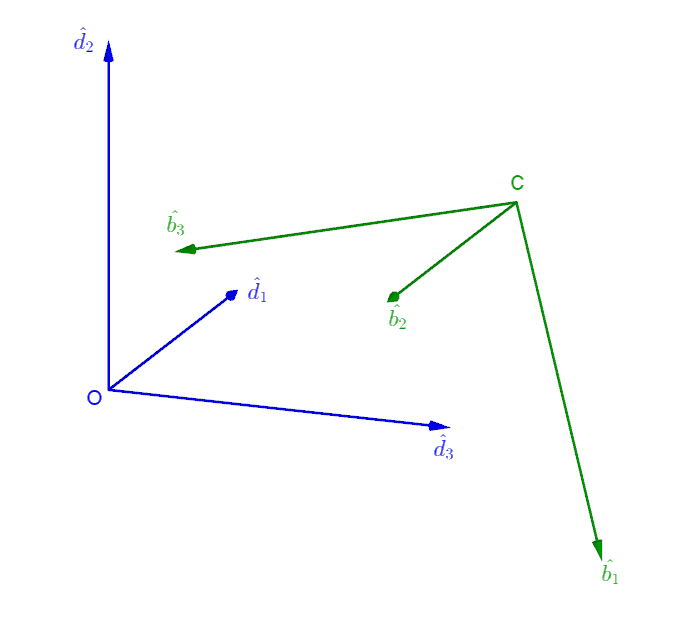
\includegraphics[width=0.7\linewidth]{images/WeltKordSys.png}
%		\captionof{figure}{Weltkoordinatensystem $(O,\delta)$ mit $\delta = (\hat{d_1},\hat{d_2},\hat{d_3})$ und Kamerakoordinatensystem  $(C,\beta)$ mit $\beta = (\hat{b_1},\hat{b_2},\hat{b_3})$ }
%		\label{fig:Koordinatensysteme1}
%	\end{minipage}\\ \\
	
	
Zunächst wird eine sogenannte Koordinatisierung von Punkten im Weltkoordinatensystem vorgenommen. Ein Punkt $P_\delta$ bezüglich des Weltkoordinatensystems wird dann wie folgt beschrieben.

	
	\begin{gather}
	P_\delta = O + p_{1\delta}\hat{d_1} + p_{2\delta}\hat{d_2} + p_{3\delta}\hat{d_3}\\
	\leadsto P_\delta = (p_{1\delta},p_{2\delta},p_{3\delta})^T = \begin{pmatrix} p_{1\delta} \\ p_{2\delta} \\ p_{3\delta} \end{pmatrix}
	\end{gather}
	
Um das Koordinatentupel in einem projektiven Raum darstellen zu können, wird es projektiv erweitert. Die Entstehenden projektiv erweiterten Koordinaten werden als homogene Koordinaten bezeichnet. Ein Punkt $P_\delta$ bezüglich des Weltkoordinatensystems wird um eine vierte homogene Komponente erweitert. Diese kann einen Wert zwischen 0 und 1 annehmen. Nimmt die Komponente den Wert 0 an, so handelt es sich um einen Fernpunkt, sprich der Punkt liegt im unendlichen.
%wird dann zum Zweck der Einführung homogener Objekte projektiv Erweitert.
	
	\begin{gather}
	P_\delta = \begin{bmatrix} p_{1\delta} \\ p_{2\delta} \\ p_{3\delta} \\1 \end{bmatrix} = \left\{ k \begin{bmatrix} p_{1\delta}\\p_{2\delta}\\p_{3\delta}\\1 \end{bmatrix} \in \mathbb{R} ^4 |  k \in \mathbb{R}\right\}\\
	\begin{bmatrix}\lambda p_{1\delta}\\ \lambda p_{2\delta} \\ \lambda p_{3\delta} \\ 1 \end{bmatrix} = \begin{bmatrix}p_{1\delta} \\ p_{2\delta} \\ p_{3\delta} \\ 1\end{bmatrix} \text{für} \; \lambda \ne 0
	\end{gather}


Ein Punkt $P_\beta$ bezüglich des Kamerakoordinatensystem wird im Vergleich wie folgt beschrieben.
	
	\begin{gather}
	P_\beta = C + p_{1\beta}\hat{b_1} + p_{2\beta}\hat{b_2} +  p_{3\beta}\hat{b_3}\\
	P_\beta = \begin{pmatrix} p_{1\beta} \\  p_{2\beta} \\ p_{2\beta}\end{pmatrix}
	\end{gather}\\
	
	Zwischen den beiden Koordinatensystemen	$(O,\delta)$  und $(C,\beta)$ werden die folgenden Beziehungsgleichungen aufgestellt. 
	
	\begin{gather}
	C_\beta = O_\delta + C_{\beta,1}\hat{d_1} +C_{\beta,2}\hat{d_2} + C_{\beta,3}\hat{d_3}\\
	\hat{b_1} = b_{11}\hat{d_1} +  b_{12}\hat{d_2} +  b_{13}\hat{d_3}\\
	\hat{b_2} = b_{21}\hat{d_1} +  b_{22}\hat{d_2} +  b_{23}\hat{d_3}\\
	\hat{b_3} = b_{31}\hat{d_1} +  b_{32}\hat{d_2} +  b_{33}\hat{d_3}
	\end{gather}
	
	Diese Beziehungsgleichungen werden in Gleichung 3.1 eingesetzt.
	
	\begin{gather}
	\begin{split}
	P_\delta = O + (C_{\beta,1} + p_{1\beta}b_{11} +  p_{2\beta}b_{21} + p_{3\beta}b_{31}) \cdot \hat{d_1}\\
	+(C_{\beta,2} + p_{1\beta}b_{21} +  p_{2\beta}b_{22} + p_{3\beta}b_{32} )\cdot \hat{d_2}\\
	+ (C_{\beta,3} + p_{1\beta}b_{31} +  p_{2\beta}b_{23} + p_{3\beta}b_{33} )\cdot \hat{d_3}
	\end{split}
	\end{gather}
	
Aus Gleichung 3.11 wird ein Gleichungssystem in der Form von Gleichung 3.12 aufgestellt und gelöst.
	
	\begin{gather}
	\begin{split}
	p_{1\delta} = C_{\beta,1} + (C_{\beta,1} + p_{1\beta}b_{11} +  p_{2\beta}b_{21} + p_{3\beta}b_{31} \\
	\leadsto \: p_{1\delta} - C_{\beta,1} =  (C_{\beta,1} + p_{1\beta}b_{11} +  p_{2\beta}b_{21} + p_{3\beta}b_{31})
	\end{split}
	\end{gather}
	
Wenn $P_\beta$ gegeben ist, erhält man auf diese Weise direkt $P_\delta$. Wenn jedoch  $P_\delta$  gegeben ist, so muss das in Gleichung 3.13 aufgestellte lineare Gleichungssystem gelöst werden.
	
	\begin{gather}
	\begin{bmatrix}b_{11} & b_{21} & b_{31}\\
	b_{12} & b_{22} & b_{32}\\
	b_{13} & b_{23} & b_{33}
	\end{bmatrix} 
	\begin{pmatrix}
	p_{1\beta}\\p_{2\beta}\\ p_{3\beta}
	\end{pmatrix} = 
	\begin{pmatrix}
	p_{1\delta} - C_{\beta,1}\\
	p_{2\delta} - C_{\beta,2}\\
	p_{3\delta} - C_{\beta,3}
	\end{pmatrix}
	\end{gather}
	
 Wenn $(C,\beta)$ ein kartesisches Koordinatensystem ist, so ist die entstehende  koeffizientenmatrix $D_\beta$ orthogonal und es gilt \ensuremath{D_\beta^{-1} = D_\beta^T}. 
	\begin{gather}
	D_\beta^{T} = 
	\begin{bmatrix}b_{11} & b_{12} & b_{13}\\
	b_{21} & b_{22} & b_{23}\\
	b_{31} & b_{32} & b_{33}
	\end{bmatrix} \\
	\begin{split}
	\leadsto \: \begin{pmatrix}
	p_{1\beta}\\p_{2\beta}\\ p_{3\beta}
	\end{pmatrix}
	= D_\beta^T 
	\begin{pmatrix}
	p_{1\delta} - C_{\beta,1}\\
	p_{2\delta} - C_{\beta,2}\\
	p_{3\delta} - C_{\beta,3}
	\end{pmatrix}
	\end{split} 
	\end{gather}
	
Handelt es sich um kein kartesisches Koordinatensystem, so muss lediglich die Inverse \ensuremath{D_\beta^{-1}} anstatt der Transponierten \ensuremath{D_\beta^T} gebildet und wie gehabt verfahren werden. Im folgenden wird noch einmal kompakt und in einer symbolischen Schreibweise die Transformation von Welt- in Kamerakoordinaten  festgehalten. Einmal wird wie bereits angefangen mit Spaltenvektoren gearbeitet, das selbe Verfahren wird dann noch einmal mit Zeilenvektoren dargestellt.  Beide Ansätze funktionieren nach dem selben Prinzip, der einzige Unterschied ist die Darstellung der Matrizen. Es ist jedoch gerade wenn man mit Programmen wie Beispielsweise \textit{Matlab} arbeitet wichtig zu wissen welche Darstellung benutzt wird und worin sie sich unterscheiden. Auf diese weise passieren keine Fehler beim Interpretieren der späteren Resultate. \textit{MatLab} arbeitet beispielsweise mit Spaltenvektoren, während im entstandenen Algorithmus dieser Arbeit mit Zeilenvektoren gearbeitet wurde. Zunächst wird also weiter mit Spaltenvektoren verfahren. Zur Erinnerung, es gilt, dass $\beta = (\hat{b_1},\hat{b_2},\hat{b_3},C)$ durch Rotation $D$ aus $\delta = (\hat{d_1},\hat{d_2},\hat{d_3})$ entstanden ist. Der Ursprung des Kamerakoordinatensystems ist bezüglich des Ursprungs des Weltkoordiantensystems verschoben. Zur Rotation des Koordinatesystems muss also auch noch eine Tranlation des Ursprungs durchgeführt werden. Der Translationsvektor ist gleich den Koordinaten des Ursprungs des Kamerakoordinatensystem $\vec{V} = C_\beta = (C_{\beta,1}, C_{\beta,2}, C_{\beta,3})^T$. Die Transformationsmatrix welche aus der Rotation $D$ und dem Translationsvektor $\vec{V}$ ensteht, wird im weiteren Verlauf mit $R$ bezeichnet.

%Da es sich aber in einem nicht-kartesischen Koordinatensystem nicht um eine orthogonale Drehmatrix handelt wird die Rotation \textit{R} in diesem Beispiel als Transformationsmatrix \textit{C} gekennzeichnet.
% Somit soll gekennzeichnet werden, dass die Transformation unabhängig der Definition ihres ausgehenden Koordinatensystem allgemein formuliert werden kann. Es gilt für die Transformation von Welt- in Kamerakoordinaten ausgehend von Spaltenvektoren folgendes.
	
	\begin{gather}
	\begin{pmatrix}
	\hat{b_1}\\
	\hat{b_2}\\
	\hat{b_3}\\
	C_\beta
	\end{pmatrix} = 
	\begin{bmatrix}
	b_{11} & b_{21} & b_{31} & 0\\
	b_{12} & b_{22} & b_{32} & 0\\
	b_{13} & b_{23} & b_{33} & 0\\
	C_{\beta,1} & C_{\beta,2} & C_{\beta,3} & 1
	\end{bmatrix}
	\begin{pmatrix}
	\hat{d_1}\\
	\hat{d_2}\\
	\hat{d_3}\\
	O_\delta
	\end{pmatrix}\\
	D^T = D^{-1}= \begin{bmatrix}
	b_{11} & b_{12} & b_{13} \\
	b_{21} & b_{22} & b_{23} \\
	b_{31} & b_{32} & b_{33} 
	\end{bmatrix}\\
	D = \begin{bmatrix}
	b_{11} & b_{21} & b_{31} \\
	b_{12} & b_{22} & b_{32} \\
	b_{13} & b_{23} & b_{33} 
	\end{bmatrix}
	\end{gather}

Für eine Rücktransformation von Kamera in Weltkoordinaten muss die Inverse von $D$ gebildet werden.
Außerdem muss der Translationsvektor $\vec{V}$ ebenfalls mit dieser Inversen multipliziert werden, um diesen ebenfalls in das Zielkoordinatensystem zu überführen.
	
	
	\begin{gather}
	\leadsto \: \begin{pmatrix}
	\hat{d_1}\\
	\hat{d_2}\\
	\hat{d_3}\\
	O_\delta
	\end{pmatrix} = 
	\begin{bmatrix}
	b_{11} & b_{21} & b_{31} & 0\\
	b_{12} & b_{22} & b_{32} & 0\\
	b_{13} & b_{23} & b_{33} & 0\\
	&-(	C_{\beta,1}, C_{\beta,2}, C_{\beta,3})C^{-1}& & 1
	\end{bmatrix}
	\begin{pmatrix}
	\hat{b_1}\\
	\hat{b_2}\\
	\hat{b_3}\\
	C_\beta
	\end{pmatrix}
	\end{gather}
	
	
Das selbe Verfahren mit Zeilenvektoren führt zu den Gleichungen 3.20 und 3.21.
	
%	Die  Rücktransformation von Kamera- in Weltkoordinaten beinhaltet mit Spaltenvektoren dargestellt also folgendes:
%	
%	\begin{gather}
%	(a,b,c,1) 
%	\begin{bmatrix}
%	c_{11} & c_{12} & c_{13} & 0\\
%	c_{21} & c_{22} & c_{23} & 0\\
%	c_{31} & c_{32} & c_{33} & 0\\
%	o_{c,1} & o_{c,2} & o_{c,3} & 1
%	\end{bmatrix}
%	= (0,0,0,1)
%	\end{gather}
	
%Die Formel 2.21 zeigt die selbe Transformation nur werden die Koordinatensysteme als Zeilenvektoren dargestellt.

	\begin{gather}
	(\hat{b_1}, \hat{b_2}, \hat{b_3}, C_\beta) = (\hat{d_1},\hat{d_2}, \hat{d_3}, O) \cdot
	\begin{bmatrix} 
	b_{11} & b_{21} & b_{31} & C_{\beta,1}\\
	b_{12} & b_{22} & b_{23} & C_{\beta,2}\\
	b_{13} & b_{32} & b_{33} & C_{\beta,2}\\
	0           &       0       &   0         & 1   
	\end{bmatrix}
	\end{gather}	
	
	Daraus folgt, dass für den Fall der Rücktransformation gilt:
	
	\begin{gather}
	\leadsto \: \begin{pmatrix}
	\hat{d_1},\hat{d_2},\hat{d_3},O
	\end{pmatrix} = 
	\begin{bmatrix}
	b_{11} & b_{12} & b_{13} & \\
	b_{21} & b_{22} & b_{23} &  -\begin{pmatrix}
C_{\beta,1}\\
C_{\beta,2}\\
C_{\beta,3}
	\end{pmatrix}C^{-1}\\
	b_{31} & b_{32} & b_{33} & \\
	0&0&0 & 1
	\end{bmatrix}
	\begin{pmatrix}
	\hat{b_1},\hat{b_2},\hat{b_3},C_\beta
	\end{pmatrix}
	\end{gather}	



\section{Aubau der Koordinatenssysteme}

		
Für die geplante Stereoanalyse werden insgesamt sieben verschiedene Koordinatensysteme definiert. Das Weltkoordinatensystem $(O,\delta)$ und zwei Kamerakoordinatensysteme $(C,\beta)$, welche alle drei zu den dreidimensionalen Koordinatensystemen gehören. Des Weiteren gibt noch vier zweidimensionale Koordinatensysteme. Zum einen die Bildebenenkoordinatensystem $(I,\tau)$ und $(I',\tau')$ und die Sensorkoordinatensystem $(S,\sigma)$ und $(S',\sigma')$. Alle Koordinatensysteme sind innerhalb dieser Masterarbeit als kartesische, rechtsdrehende Koordinatensysteme festgelegt. Abbildung \ref{fig:KoordinatensystemeUeberblick} zeigt als Übersicht die Koordinatensysteme von einer Kamera ausgehend im Überblick. \\

%	\begin{minipage}{\linewidth}
%	\centering
%	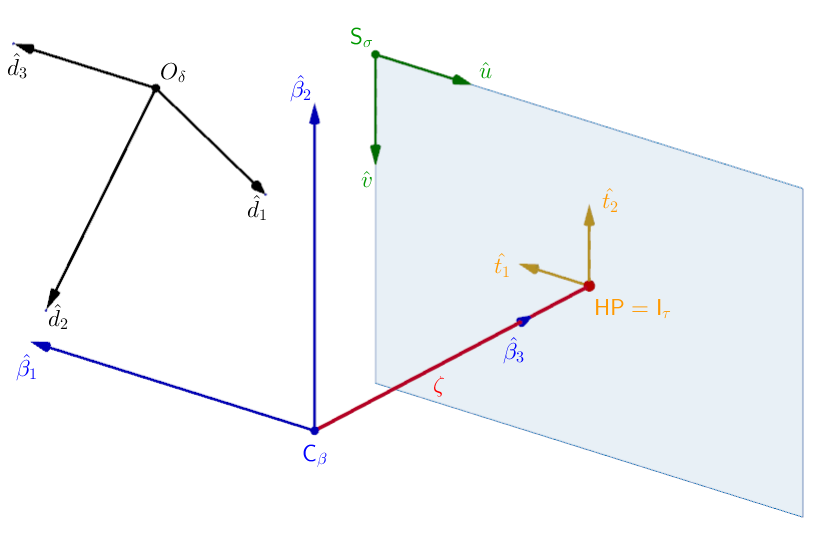
\includegraphics[width=0.8\linewidth]{images/UebersichtKoordinatensysteme_beschriftet.png}
%	\captionof{figure}{Koordinatensysteme von einer Kamera aus im Überblick. Das Weltkoordinatensystem $(O,\delta)$ ist Deckungsgleich mit dem Kamerakoordinatensystem $(C,\beta)$}
%	\label{fig:KoordinatensystemeUeberblick}
%\end{minipage}\\ \\

%
%Grundlegend muss erst einmal festgelegt werden, welche Orientierungen die Koordinatensysteme haben sollen. Die Arbeit und auch die entstanden Algorithmen basieren auf rechtsdrehenden Systemen. Die Möglichkeit linksdrehende Systeme zu benutzen, ist aus dem entstandenen Algorithmus nicht ausgeschlossen, jedoch ist es für die spätere Deutung und Interpretation der Resultate wichtig im Vorhinein definiert zu haben, wie die Orientierung der einzelnen Koordinatensysteme ist. 


Nachdem die einzelnen Koordinatensysteme definiert sind, soll symbolisch die Projektion eines Objekts  aus dem 3D-Raum auf den 2D-Sensor aufgezeigt werden. Für die Transformation der Weltkoordinaten in Kamerakoordinaten gilt, dass $[\hat{d_1}\,\hat{d_2}\,\hat{d_3}\,1] \cdot R = [\hat{b_1}\,\hat{b_2}\, \hat{b_3}\, 1]$, wobei $R$ eine Tranformationsmatrix ist, wie sie im vorherigen Abschnitt eingeführt wurde. $R=[D|V]$, wobei $D$ eine $3 \times 3$-Rotationsmatrix darstellt und $V$ die Tranlationskomponente beschreibt. Der Translationsvektor \ensuremath{\vec{V}} besteht aus den Koordinaten des Projektionszentrums \textit{C}. Es gilt also $\vec{V} = C \leadsto \vec{v} = \begin{pmatrix}	C_{\delta,1}\\C_{\delta,2}\\C_{\delta,3}\end{pmatrix}$. 


(BEISPIEL BILDAUFNAHME IM ROTIERTEN SYSTEM)
 
\begin{gather} 		
(\hat{b_1}, \hat{b_2}, \hat{b_3},1)=(\hat{d_1},\hat{d_2},\hat{d_3},1) \cdot
\begin{bmatrix}
&  &  &C_{\delta,1} \\
&  [D]&  &C_{\delta,2} \\ 
&  &  &C_{\delta,3} \\
0&0&0 & 1
\end{bmatrix}	
\end{gather}

Ein Punkt $M_\delta$ Mit $M_\delta=[X_\delta,Y_\delta,Z_\delta,1]$ wird mit der soeben aufgestellten Transformationmatrix R=[D|V] zu einem Punkt $M_\beta$ transformiert.

\begin{gather}
M_\beta = M_\delta \cdot R\\
\begin{bmatrix}
X_\beta& Y_\beta& Z_\beta&1\\
\end{bmatrix} = 
\begin{bmatrix}
X_\delta& Y_\delta& Z_\delta&1\\
\end{bmatrix} \cdot
\begin{bmatrix}
	&  &  &C_{\delta,1} \\
	&  [D]&  &C_{\delta,2} \\ 
	&  &  &C_{\delta,3} \\
	0&0&0 & 1
\end{bmatrix}	
\end{gather}


Nach der Transformation eines Punkte $M_\delta$ in 3D-Kamerakoordinaten zu $M_\beta$, erfolgt nun die Porjektion des 3D-Kamerapunktes $M_\beta$ in die 2D-Bildebene zu $m_\tau$. Für die Projektion wird eine $3 \times 3$-Kameramatrix $K$ aufgestellt.  Es wird angenommen, dass $\zeta_x = \zeta_y =\zeta$
%Im nächsten Schritt müssen die Transformierten Kamerakoordinaten noch mit einer entsprechenden Kameramatrix $K$, welche die Punkte aus dem Kamerakoordinatensystem $(C,\beta)$ auf das Koordinatensystem der Bildebene $(I,\tau)$ mit $\tau = (t_1,t_2)$ projiziert, verrechnet werden. Hierzu muss eine entsprechende Kameramatrix $K$ aufgestellt werden. $\zeta$ erhält als Wert den Abstand des Projektionszentrums $Z$ zur Bildebene $I$.

	\begin{gather}
K = 
\leftidx{_{{I_\beta}}}{\begin{bmatrix}
	\pi
	\end{bmatrix}}{_{{C_\beta}}}
=
\begin{bmatrix}
\zeta&0&0&0\\
0&\zeta&0&0\\
0&0&\zeta&0\\
0&0&1&0
\end{bmatrix}\\
\begin{bmatrix}
\zeta&0&0&0\\
0&\zeta&0&0\\
0&0&\zeta&0\\
0&0&1&0
\end{bmatrix}
\begin{bmatrix}
X_\beta\\Y_\beta\\Z_\beta\\1
\end{bmatrix} =
\begin{pmatrix}
\zeta X\\ \zeta Y\\ \zeta Z \\ Z
\end{pmatrix}
=
\begin{bmatrix}
\zeta \frac{X}{Z}\\ \zeta \frac{Y}{Z}\\ \zeta  \\ 1
\end{bmatrix}
\end{gather}

Für die Koordinaten der Bildebene $I_\beta$ ergeben sich dann aus den Kamerakoordinaten $[\zeta \frac{X}{Z},\zeta\frac{Y}{Z},\zeta,1]^T$. Da die Koordinaten momentan noch in homogenen 3D-Koordinaten angegeben sind, aber das Bildebenenkoordinatensystem ein 2D-Koordinatensystem muss der Tiefenwert noch eliminiert werden. $\zeta$ gibt den Abstand von $C$ zu $I$ an, somit sind die 2D-Bildkorrdinaten des die Bildebenenkooridnatensystem  $[\zeta \frac{X}{Z},\zeta\frac{Y}{Z},1]^T = [X_\tau, Y_\tau,1]$. Zuletzt folgt in der Transformationskette noch die Transformation der Bildebenenkoordinaten in die Sensorkoordinaten mit dem Sensorkoordinatensystem $(S,\sigma)$ mit $\sigma = (\hat{u},\hat{v})$. $\hat{u}$ und $\hat{v}$ definieren die geometrische Beschaffung der Pixel, sie werdn auch als Vektoren $\vec{u}$ und $\vec{v}$ angegeben, somit muss das Sensorkoordinatensystem nicht zwangsläufig ein kartesisches Koordinatensystem sein. Die Werte $V_{\sigma,1}$ und $V_{\sigma,2}$ stehen für die Verschiebung des Koordinatensystemursprungs Hauptunkt auf der Bildebene in eine der Ecken der Bildebene.
		
		\begin{gather}
		\vec{u} = u_1 \hat{t_1} + u_2 \hat{t_2}\\
		\vec{v} = v_1 \hat{t_1} + v_2 \hat{t_2}\\
		S_\sigma = I_\tau +V_{\sigma,1} \hat{t_1} + V_{\sigma,2} \hat{t_2}\\
		\begin{pmatrix}
		\vec{u}, \vec{v}, 1
		\end{pmatrix}		
		=
		\begin{pmatrix}
		\hat{t_1}, \hat{t_2}, 1
		\end{pmatrix}\cdot	
		\begin{bmatrix}
		u_1&v_1&V_{\sigma,1}\\u_2&v_2&V_{\sigma,2}\\0&0&1\\
		\end{bmatrix}
		\end{gather}
		
		Der Koordinatenwechsel von Bildebenenkoordinaten in Sensorkoordinaten wird noch einmal Symbolisch veranschaulicht.	 
		
		Es wird ein Punkt $X_\sigma=\begin{pmatrix}
		a\\b\\1
		\end{pmatrix}$. In Sensorkoordinaten definiert. Die Transfomationsmatrix $M = \begin{bmatrix}
	u_1& v_1\\
	u_2& v_2
\end{bmatrix}$ beinhaltet statt einer Rotation eine Skalierung der Koordinatenwerte auf die Koordinaten des Sensorkoordinatensystems. Mit $M$ lässt sich wieder eine Projektionsmatrix $P$ aus einer Abbildungsmatrix $K$ mit einer Transformationsmatrix $M$ aufstellen. Ein Punkt $X_\tau$ wird in einen Punkt $X_\sigma$ transformiert.
	
		\begin{gather}
		X_\sigma =
		\begin{bmatrix}
		&  & \\
		&\begin{bmatrix}
		u_1& v_1\\
		u_2& v_2
		\end{bmatrix}^{-1}  & -M^{-1}\begin{pmatrix}
		V_{\sigma,1}\\V_{\sigma,2}
		\end{pmatrix} \\ 
		&  & \\
		0&0 & 1
		\end{bmatrix}
		\cdot
		X_\tau	
		\end{gather}\\
		
		 Die Projektionsmatrix $P$, welche die Kamerakoordinaten in Sensorkoordinaten überführt, wird dann wie folgt aufgebaut:\\
		
 	\begin{gather} 		
 		P 
		=
		\begin{bmatrix}
		&&\\
		&M^{-1}& -M\begin{pmatrix}V_{\sigma,1}\\V_{\sigma,2}\end{pmatrix}^{-1}\\
		&&\\
		0&0&1
		\end{bmatrix}
		\cdot
		\begin{bmatrix}
		-\zeta&0&0&0\\
		0&-\zeta&0&0\\
		0&0&1&0
		\end{bmatrix}
		=
		\begin{bmatrix}
		&&&0\\
		&-\zeta M^{-1}& -M\begin{pmatrix}V_{\sigma,1}\\V_{\sigma,2}\end{pmatrix}^{-1}&0\\
		&&&\\
		0&0&1&0
		\end{bmatrix}
		\end{gather}
	
%
%		
%		Zur Verdeutlichung folgen nun noch zwei Beispiele. Es werden $\vec{u}$ und $\vec{v}$, sowie $z_1$ und $z_2$ mit Werten versehen. $p$ entspricht symbolisch einem \textit{Pixelpitch}-Wert. Mit \textit{Pixelpitch} wird der direkte Abstand der Pixel auf Bildsensoren zwischen Pixelmitte zu Pixelmitte bezeichnet.\\
		
%		\underline{Beispiel 1:}\\
%		
%		$\vec{u} = 1pt_1 $\\
%		$\vec{v} = 2pt_2 $\\
%		$ p_1 = 15, p_2 = 20$\\
%		
%		Für die Projektionsmatrix $P$ ergibt sich somit:
%		
%		\begin{gather}
%		S_\sigma = I_\tau - \vec{u} - \vec{v} \leadsto S_\sigma = I_\tau -15 t_1 - 20 t_2\\	
%		M= 
%		\begin{bmatrix}
%		1&0\\
%		0&2
%		\end{bmatrix}
%		\leadsto
%		M^{-1}=\begin{bmatrix}
%		\frac{1}{p}&0\\
%		0&\frac{1}{2p}
%		\end{bmatrix}\\
%		K =
%		\leftidx{_{S_\sigma}}{\begin{bmatrix}
%				\pi
%		\end{bmatrix}}{_{I_\tau}} = 	
%		\begin{bmatrix}
%		\frac{-\zeta}{p}&0&15&0\\
%		0&\frac{-\zeta}{p}&20&0\\
%		0&0&1&0
%		\end{bmatrix}
%		\end{gather}\\
%		
%	 	\underline{Beispiel 2:}\\
%		
%		$\vec{v} = 1pt_1+2pt_2$\\
%		$\vec{u} = 1pt_1$\\
%		$ z_1 = 10, z_2 = 5$\\
%		
%		\begin{gather}
%		M=\begin{bmatrix}
%		1&1\\
%		0&2
%		\end{bmatrix} \leadsto 
%		M^{-1} =
%		\begin{bmatrix}
%		1&-\frac{1}{2}\\
%		0&\frac{1}{2}
%		\end{bmatrix} \\
%		K = \leftidx{_{S_\sigma}}{\begin{bmatrix}
%				\pi
%		\end{bmatrix}}{_{C_\beta}}
%		= 
%		\begin{bmatrix}
%		\frac{-\zeta}{p}&\frac{-\zeta}{2p}&10&0\\
%		0&\frac{-\zeta}{p}&5&0\\
%		0&0&1&0
%		\end{bmatrix}\\
%		= [K|0]
%		\end{gather}
		
		Die symbolische Darstellung der Projektionsmatrix von Welt in Sensorkoordinaten $	P = \leftidx{_{S_\sigma}}{\begin{bmatrix}
			\pi
			\end{bmatrix}}{_{O_\delta}}$ fügt sich somit aus dem vorhergehenden Abbildungsmatrix 
		K = $\leftidx{_{S_\sigma}}{\begin{bmatrix}
				\pi
		\end{bmatrix}}{_{C_\beta}}$ mit der Tranformationsmatrix $R$ zusammen.
		
		\begin{gather}
		\leftidx{_{S_\sigma}}{\begin{bmatrix}
			\pi
			\end{bmatrix}}{_{O_\delta}}
		=
		\leftidx{_{S_\sigma}}{\begin{bmatrix}
			\pi
			\end{bmatrix}}{_{C_\beta}}
		\cdot
		\begin{bmatrix}
		&&&\\
		&[C]^{-1}&& -[C]^{-1} Z\\
		&&&\\
		0&0&0&1\\
		\end{bmatrix}
		\end{gather}\\
		
	Somit ist die Transformations-Pipeline eines Punkte im Raum auf den Sensor einer Kamera am Ende. 
Zum Schluss hier noch einmal zum Vergleich die Darstellung der Projektionsmatrix $P$ aus \textit{Hartley\&Zisserman}\cite{HZ}. Zu beachten ist hier, dass im \textit{Hartley\&Zisserman} $R$ für $[R]^{-1}$ steht\cite{HZ}.
		
		\begin{gather}
		\begin{split}	
		P=
		[K|0] \begin{bmatrix}
		&&&\\
		&R&&-RZ\\
		&&&\\
		0&0&0&1\\
		\end{bmatrix}\\
		=[KR|-KRZ] 	= KR[I_{3x3}|-Z]
		\end{split}
		\end{gather}
